\documentclass{beamer}
\usepackage{xcolor}
% \usetheme{Marburg}
\usecolortheme{orchid}
\usepackage{pifont}
\usepackage{nicefrac}
\usepackage{csquotes}
\usepackage{changepage}
\usepackage{cancel} 
\newcommand{\crossout}[2][red]{%
  \begin{tikzpicture}[baseline=(texte.base)]
    % Nœud pour le texte
    \node[inner sep=0pt, outer sep=0pt] (texte) {#2};
    % Dessiner la croix (deux lignes diagonales)
    \draw[overlay, #1, line width=0.5pt] 
      (texte.north west) -- (texte.south east); % Ligne diagonale 1
    \draw[overlay, #1, line width=0.5pt] 
      (texte.north east) -- (texte.south west); % Ligne diagonale 2
  \end{tikzpicture}%
}
\usepackage[ 
backend=biber,
style=alphabetic,
]{biblatex}
\addbibresource{main.bib}
\usepackage{hyperref, xcolor, cmbright,diagbox,colortbl,tikz,graphicx,algorithm2e,cancel,verbatim, graphicx,
listings,float,amsmath,amssymb,array,subfiles,bussproofs,
rotating,MnSymbol,hyperref,mathtools,subcaption,caption}
\newtheorem{proposition}{Proposition}
\usetikzlibrary{overlay-beamer-styles}
\usetikzlibrary{automata, positioning,graphs,shapes, arrows, calc}

\newcommand{\set}[1]{\{#1\}}
\newcommand{\vertex}[2]{%
  \begin{tikzpicture}[baseline=-1ex]%
    \node [rectangle,rounded corners=2mm,inner sep=0.5mm,fill=#2] {$#1$};%
  \end{tikzpicture}%
}
\newcommand{\graphbox}[8]{
  \begin{scope}[xshift=#2,yshift=#3]
    \draw [rounded corners=2mm] (0,0) rectangle (#4,-#5);
    \node at (0,0mm) [anchor=north west,inner sep=1mm] {#1};
    \begin{scope}[xshift=#4/2+#6,yshift=#7] 
    #8
    \end{scope}
  \end{scope}
}

\newcommand{\opn}[1]{\operatorname{#1}}

\graphicspath{ {.} }

\title{Termination of Graph Rewriting
using Weighted Type Graphs
over Non-well-founded Semirings}
\setbeamertemplate{footline}[frame number]
\begin{document}
% \date{\today}
\date{}

\institute[VFU] % (optional)
{
    Qi QIU \\
	Supervisor: Xavier URBAIN\\
	Universite Claude Bernard Lyon 1, CNRS, INSA Lyon,\\ LIRIS, UMR5205, 69622 Villeurbanne, France \\
    Univ. Grenoble Alpes, CNRS, Grenoble INP,\\
               LIG, 38000 Grenoble, France\\
	% Projet SAPPORO
}

\maketitle
% \begin{frame}
%   \begin{itemize}
%     \item Termination by constructing a weighted type graph over three concrete semirings on natural numbers
%     \item weighted type graph construction in literature
%     \item problem of complexity
%     \item Question: can we use weighted type graphs over real numbers to prove termination of DPO rewriting systems?
%     \item termination by interpretation : homomorphism to a well-founded order
%     \item weighted type graph method : associate a natural number to each graph 
%     \item weighted type graph method : weighted type graph
%     \item weighted type graph method : weight of graph morphism
%     \item weighted type graph method : weight of graph
%     \item lemm decomposition
%     \item decreasing step : example 0.25
%     \item reduced complexity
%   \end{itemize}
% \end{frame}



\begin{frame}{Plan (for myself)}
  \begin{itemize}
    \item Termination of DPO rewriting systems
    \item Example: looping and terminating examples
    \item Type graph method in theory 
    \item Type graph method in practice and the introduction of the main problem
    \item Morphism weight (by a example)
    \item Graph weight (by a example)
    \item A condition that weighted type graphs must satisfy
    \item Rule $\varphi$
    \item Example with rule $\varphi$
    \item Sufficient condition for termination using weighted type graph
    \item Sufficient condition simplified
    \item Example
    \item Example : termination of rule $\varphi$
    \item How to find a weighted type graph in practice
    \item Experimental results
    \item Acknowledgements
    \item Conclusion
  \end{itemize}
\end{frame}

\begin{frame}{DPO graph rewriting}
\begin{adjustwidth}{-0.5cm}{0cm}
  \begin{itemize}
      \item Finite directed multigraphs with edge labels from a finite set $\Sigma$.
      %   \begin{center}
      %     \resizebox{0.5\textwidth}{!}{
      %     \begin{tikzpicture}
      %         \graphbox{\(\)}{00mm}{-20mm}{35mm}{15mm}{2mm}{-5mm}{ 
      %             \coordinate (o) at (-2mm,-2mm); 
      %             \node[draw,circle] (l1) at ($(o)+(-10mm,0mm)$) {};
      %             \node[draw,circle] (l3) at ($(l1)+(1,0)$) {};
      %             \node[draw,circle] (l4) at ($(l1)+(2,0)$) {};
      %             \draw[->] (l1) edge[bend right]  node[midway,below] {a} (l3);
      %             \draw[->] (l1) edge[bend left] node[midway,above] {a}  (l3);
      %             \draw[->] (l3) -- (l4) node[midway,above] {b};
      %             % \draw[->] (l4) -- (l2) node[midway,above] {a};
      %         }   
      %     \end{tikzpicture} 
      % }
      % \end{center}
      \item Graph morphism $h : G \rightarrow H$ 
      % : function from graph $K$ to graph $L$ that preserves the structure of the graphs.
         \begin{center}
          \resizebox{0.8\textwidth}{!}{
          \begin{tikzpicture}
            \graphbox{\( G \)}{00mm}{-20mm}{45mm}{25mm}{2mm}{-10mm}{
                \coordinate (o) at (-5mm,-8mm); 
                \node[draw,circle] (l1) at ($(o)+(-10mm,0mm)$) {1};
                \node[draw,circle] (l2) at ($(l1)+(3,0)$) {2};
                \node[draw,circle] (l3) at ($(l1)+(1,0)$) {3};
                \node[draw,circle] (l4) at ($(l1)+(2,0)$) {4};
                \draw[->] (l1) -- (l3) node[midway,above] {a};
                \draw[->] (l3) -- (l4) node[midway,above] {b};
                \draw[->] (l4) -- (l2) node[midway,above] {a};
            }  
            \graphbox{\( H \)}{52mm}{-20mm}{50mm}{25mm}{2mm}{-10mm}{
                \coordinate (o) at (-5mm,-8mm); 
                \node[draw,circle] (l1) at ($(o)+(-1,0mm)$) {1};
                \node[draw,circle] (l2) at ($(l1)+(3,0)$) {2};
                \node[draw,circle] (l3) at ($(l1)+(1.5,0)$) {3\ 4};
                \draw[->] (l1) edge node[midway,above] {a} (l3);
                \draw[->] (l3) edge [loop above] node[midway,above] {b} (l3) ;
                \draw[->] (l3) -- (l2) node[midway,above] {a};
            }      
            \node () at (48mm,-30mm) {$\overset{h}{\rightarrow}$};
        \end{tikzpicture}
          }
         \end{center}

      \item Rules $\varphi = (L \overset{l}{\leftarrow} K \overset{r}{\rightarrow} R)$ consist of two graph morphisms $l: K \to L$ and $r: K \to R$.
      \item Rewriting steps $G \Rightarrow_\varphi H$ are double-pushouts:
         \begin{center}
          \resizebox{0.45\textwidth}{!}{
              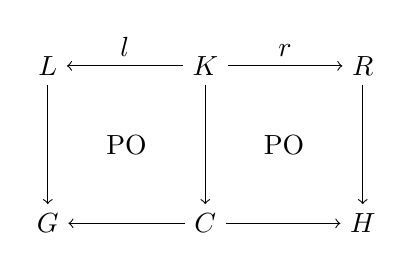
\begin{tikzpicture}
                    \node (I) at (0,0) {$K$};
                    \node (L) at (-2,0) {$L$};
                    \node (R) at (2,0) {$R$};
                    \node (G) at (-2,-2) {$G$};
                    \node (C) at (0,-2) {$C$};
                    \node (H) at (2,-2) {$H$};
                    \draw [->] (I) to  node [midway,above] {$l$} (L);
                    \draw [->] (I) to  node [midway,above] {$r$} (R);
                    \draw [->] (L) to node [midway,right] {} (G);
                    \draw [->] (I) to node [midway,right] { } (C);
                    \draw [->] (R) to node [midway,left] { } (H);
                    \draw [->] (C) to node [midway,above] { } (G);
                    \draw [->] (C) to node [midway,above] { } (H);
                    \node [at=($(I)!.5!(G)$)] {\normalfont PO};
                    \node [at=($(I)!.5!(H)$)] {\normalfont PO};
                  \end{tikzpicture}
          }
      \end{center}
  \end{itemize} 
\end{adjustwidth}
\end{frame} 

\begin{frame}{Termination}
  \begin{itemize}
    \item $\mathcal{R}$ : set of DPO graph transformation rules
    \item Impossible to transform any graph $G_0$ indefinitely
      \begin{center}
        $G_0 \Rightarrow_\mathcal{R} G_1 \Rightarrow_\mathcal{R} G_2 \Rightarrow_\mathcal{R} \cdots$
      \end{center}
    \item Guarantees that the non-deterministic strategy
          \begin{center}
              \textcolor{blue}{apply rules as long as possible}
          \end{center}
          returns a result on all inputs
    \item Corresponds to program termination:
          \begin{center}
            \textcolor{blue}{program halts on all inputs}
          \end{center}
    \item Undecidable in general
  \end{itemize}
\end{frame}

\begin{frame}{One-rule examples}
  Rule $\alpha$:  
  \begin{center}  
                \resizebox{0.7\textwidth}{!}{
                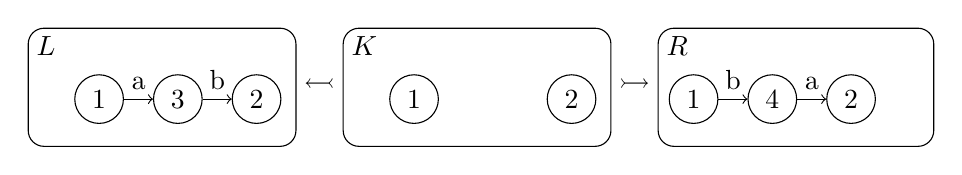
\begin{tikzpicture}
                    \graphbox{\( L \)}{0mm}{-3mm}{34mm}{15mm}{2mm}{2mm}{
                        \coordinate (o) at (0mm,-11mm); 
                        \node[draw,circle] (l1) at ($(o)+(-10mm,0mm)$) {1};
                        \node[draw,circle] (l2) at ($(l1)+(2,0)$) {2};
                        \node[draw,circle] (l3) at ($(l1) + (1,0)$) {3};
                        \draw[->] (l1) -- (l3) node[midway,above] {a};
                        \draw[->] (l3) -- (l2) node[midway,above] {b};
                    } 
            
                    \graphbox{\( K \)}{40mm}{-3mm}{34mm}{15mm}{2mm}{2mm}{
                        \coordinate (o) at (0mm,-11mm); 
                        \node[draw,circle] (l1) at ($(o)+(-10mm,0mm)$) {1};
                        \node[draw,circle] (l2) at ($(l1)+(2,0)$) {2};
                    }  
            
                    \graphbox{\( R \)}{80mm}{-3mm}{35mm}{15mm}{2mm}{2mm}{
                        \coordinate (o) at (-5mm,-11mm); 
                        \node[draw,circle] (l1) at ($(o)+(-10mm,0mm)$) {1};
                        % \node[draw,circle] (l2) at ($(l1)+(3,0)$) {2};
                        \node[draw,circle] (l3) at ($(l1) + (1,0)$) {4};
                        \node[draw,circle] (l4) at ($(l1) + (2,0)$) {2};
                        \draw[->] (l1) -- (l3) node[midway,above] {b};
                        \draw[->] (l3) -- (l4) node[midway,above] {a};
                        % \draw[->] (l4) -- (l2) node[midway,above] {a};
                    }    
                    \node () at (37mm,-10mm) {\( \leftarrowtail \)}; % K -> L
                    \node () at (77mm,-10mm) {\( \rightarrowtail \)}; % K -> R
                \end{tikzpicture}
                }
            \end{center}  

\textcolor{blue}{Looping}:
        \begin{center}
          \resizebox{0.7\textwidth}{!}{
            \tikz[baseline=-0.5ex]{ 
                \node (x) at (0,0) {$\bullet$};  
                \node (y) at (1,0) {$\bullet$};
                \node (z) at (0.5,0.86) {$\bullet$};
                \draw[->,red] (x) -- node[midway,below] {a} (y) ;
                \draw[->,red] (y) -- node[midway,right] {b} (z) ;
                \draw[->] (z) -- node[midway,left] {b} (x) ;
            } 
            $\Rightarrow$ 
            \tikz[baseline=-0.5ex]{ 
                \node (x) at (0,0) {$\bullet$};  
                \node (y) at (1,0) {$\bullet$};
                \node (z) at (0.5,0.86) {$\bullet$};
                \draw[->] (x) -- node[midway,below] {b} (y) ;
                \draw[->,red] (y) -- node[midway,right] {a} (z) ;
                \draw[->,red] (z) -- node[midway,left] {b} (x) ;
            }
            $\Rightarrow$ 
            \tikz[baseline=-0.5ex]{ 
                \node (x) at (0,0) {$\bullet$};  
                \node (y) at (1,0) {$\bullet$};
                \node (z) at (0.5,0.86) {$\bullet$};
                \draw[->,red] (x) -- node[midway,below] {b} (y) ;
                \draw[->] (y) -- node[midway,right] {b} (z) ;
                \draw[->,red] (z) -- node[midway,left] {a} (x) ;
            }
            $\Rightarrow$ 
            \tikz[baseline=-0.5ex]{ 
                \node (x) at (0,0) {$\bullet$};  
                \node (y) at (1,0) {$\bullet$};
                \node (z) at (0.5,0.86) {$\bullet$};
                \draw[->,red] (x) -- node[midway,below] {a} (y) ;
                \draw[->,red] (y) -- node[midway,right] {b} (z) ;
                \draw[->] (z) -- node[midway,left] {b} (x) ;
            }
          }
        \end{center}

          Rule $\beta$:  
  \begin{center}  
                \resizebox{0.7\textwidth}{!}{
                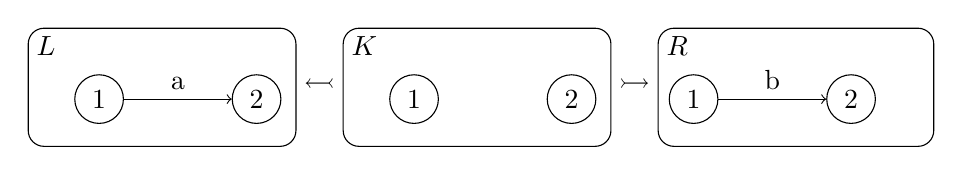
\begin{tikzpicture}
                    \graphbox{\( L \)}{0mm}{-3mm}{34mm}{15mm}{2mm}{2mm}{
                        \coordinate (o) at (0mm,-11mm); 
                        \node[draw,circle] (l1) at ($(o)+(-10mm,0mm)$) {1};
                        \node[draw,circle] (l2) at ($(l1)+(2,0)$) {2};
                        % \node[draw,circle] (l3) at ($(l1) + (1,0)$) {3};
                        \draw[->] (l1) -- (l2) node[midway,above] {a};
                    } 
            
                    \graphbox{\( K \)}{40mm}{-3mm}{34mm}{15mm}{2mm}{2mm}{
                        \coordinate (o) at (0mm,-11mm); 
                        \node[draw,circle] (l1) at ($(o)+(-10mm,0mm)$) {1};
                        \node[draw,circle] (l2) at ($(l1)+(2,0)$) {2};
                    }  
            
                    \graphbox{\( R \)}{80mm}{-3mm}{35mm}{15mm}{2mm}{2mm}{
                        \coordinate (o) at (-5mm,-11mm); 
                        \node[draw,circle] (l1) at ($(o)+(-10mm,0mm)$) {1};
                        % \node[draw,circle] (l2) at ($(l1)+(3,0)$) {2};
                        % \node[draw,circle] (l3) at ($(l1) + (1,0)$) {4};
                        \node[draw,circle] (l4) at ($(l1) + (2,0)$) {2};
                        \draw[->] (l1) -- (l4) node[midway,above] {b};
                        % \draw[->] (l4) -- (l2) node[midway,above] {a};
                    }    
                    \node () at (37mm,-10mm) {\( \leftarrowtail \)}; % K -> L
                    \node () at (77mm,-10mm) {\( \rightarrowtail \)}; % K -> R
                \end{tikzpicture}
                }
            \end{center}  

\textcolor{blue}{Terminating}: the number of edges labeled by \enquote{a} strictly decreases.
        \begin{center}
          \resizebox{0.35\textwidth}{!}{
            \tikz[baseline=-0.5ex]{ 
                \node (x) at (0,0) {$\bullet$};  
                \node (y) at (1,0) {$\bullet$};
                \node (z) at (0.5,0.86) {$\bullet$};
                \draw[->,red] (x) -- node[midway,below] {a} (y) ;
                \draw[->] (y) -- node[midway,right] {b} (z) ;
                \draw[->] (z) -- node[midway,left] {b} (x) ;
            } 
            $\Rightarrow$ 
            \tikz[baseline=-0.5ex]{ 
                \node (x) at (0,0) {$\bullet$};  
                \node (y) at (1,0) {$\bullet$};
                \node (z) at (0.5,0.86) {$\bullet$};
                \draw[->] (x) -- node[midway,below] {b} (y) ;
                \draw[->] (y) -- node[midway,right] {b} (z) ;
                \draw[->] (z) -- node[midway,left] {b} (x) ;
            }
          }
        \end{center}
\end{frame}
% \begin{frame}{Termination using Type Graphs over Real Numbers}
%   DPO Rewriting Rule on Edge-labeled Directed Graphs: 
 %     \begin{center} 
%       \resizebox{0.7\textwidth}{!}{
%       \begin{tikzpicture}
%           \graphbox{$L$}{0mm}{0mm}{34mm}{15mm}{2mm}{-5mm}{
%               \coordinate (o) at (0mm,-3mm); 
%               \node[draw,circle] (l1) at ($(o)+(-10mm,0mm)$) {1};
%               \node[draw,circle] (l2) at ($(l1)+(2,0)$) {2};
%               \node[draw,circle] (l3) at ($(l1) + (1,0)$) {3};
%               \draw[->] (l1) -- (l3) node[midway,above] {a};
%               \draw[->] (l3) -- (l2) node[midway,above] {a};
%           }     
%           \graphbox{$K$}{40mm}{0mm}{24mm}{15mm}{2mm}{-5mm}{
%               \coordinate (o) at (5mm,-3mm); 
%               \node[draw,circle] (l1) at ($(o)+(-10mm,0mm)$) {1};
%               \node[draw,circle] (l2) at ($(l1)+(1,0)$) {2};
%               % \node[draw,circle] (l3) at ($(l1) + (1,0)$) {$\ $};
%               % \draw[->] (l1) -- (l3) node[midway,above] {a};
%               % \draw[->] (l3) -- (l2) node[midway,above] {a};
%           }    
%           \graphbox{$R$}{70mm}{0mm}{45mm}{15mm}{2mm}{-5mm}{
%               \coordinate (o) at (-5mm,-3mm); 
%               \node[draw,circle] (l1) at ($(o)+(-10mm,0mm)$) {1};
%               \node[draw,circle] (l2) at ($(l1)+(3,0)$) {2};
%               \node[draw,circle] (l3) at ($(l1) + (1,0)$) {4};
%               \node[draw,circle] (l4) at ($(l1) + (2,0)$) {5};
%               \draw[->] (l1) -- (l3) node[midway,above] {a};
%               \draw[->] (l3) -- (l4) node[midway,above] {b};
%               \draw[->] (l4) -- (l2) node[midway,above] {a};
%           }    
%           \node () at (37mm,-8mm) {$\leftarrowtail$};
%           \node () at (67mm,-8mm) {$\rightarrowtail$};
%           % \draw[>->] (51mm,2mm) -- (52mm,3mm);
%       \end{tikzpicture}
%       }
%   \end{center}

%   Does the following weighted type graph witness termination?
%     \begin{center}
%         \begin{tikzpicture}
%             \graphbox{}{0mm}{0mm}{32mm}{28mm}{-10mm}{-14mm}{
%                 \node[draw,circle] (1) at (0,0) {1};
%                 \node[draw,circle] (2) at (2,0) {2};
%                 \draw[->] (1) edge[loop above] node[midway, above] {$a^{1.0}$} (1) ;
%                 \draw[->] (1) edge[loop below] node[midway, below] {$b^{1.0}$} (1) ;
%                 \draw[->] (1) edge[bend left] node[midway, above] {$a^{1.0}$}  (2)  ;
%                 \draw[->] (2) edge[bend left] node[midway, below] {$a^{1.0}$} (1)   ;
%             }
%         \end{tikzpicture}
%     \end{center}
% \end{frame}

% \begin{frame}
%   for each rewriting step $G \Rightarrow H$, $w(G) - w(H) > 1$.
% \end{frame}

\begin{frame}{Type graph method for proving termination of DPO rewriting systems on edge-labeled directed graphs}
    % Parameter : finite graph \( T \) with weights on edges

    \begin{itemize}
      \item Parameter : finite graph \( T \) with weighted edges
      \item Assigning weights $w_T(G)$ with respect to $T$ to each graphs $G$
      \item \alert{Terminating} if every step $G \Rightarrow_\mathcal{R} H$ strictly decreases the weight.
      \item \alert{Existence} of suitable $T$ : \alert{undecidable} in general
    \end{itemize}
      % \begin{itemize}
      %   \item weighted edges
      %   \item weights in $\mathbb{N}$ as superscripts of labels
      % \end{itemize} 

    % Example for the rule $\alpha$:
    % \begin{center}
    %     \begin{tikzpicture}
    %         \graphbox{}{0mm}{0mm}{32mm}{28mm}{-10mm}{-14mm}{
    %             \node[draw,circle] (1) at (0,0) {};
    %             \node[draw,circle] (2) at (2,0) {};
    %             \draw[->] (1) edge[loop above] node[midway, above] {$a^{1}$} (1) ;
    %             \draw[->] (1) edge[loop below] node[midway, below] {$b^{1}$} (1) ;
    %             \draw[->] (1) edge[bend left] node[midway, above] {$a^{1}$}  (2)  ;
    %             \draw[->] (2) edge[bend left] node[midway, below] {$a^{1}$} (1)   ;
    %         }
    %     \end{tikzpicture}
    % \end{center}
    
     

    % \textcolor{blue}{Terminating} if every step $G \Rightarrow_\mathcal{R} H$ strictly decreases the weight.

    % Undecidable in general

\end{frame}
\begin{frame}{Type graph method for proving termination of DPO rewriting systems on edge-labeled directed graphs}

    In practice

      Searching a graph \( T \) with weighted edges
      \begin{itemize}
        \item $k$ nodes
        \item no parallel edges of the same label from $\Sigma$
      \end{itemize} 
      
      Existing available tools : 
     % Interpretation method
    % Rule : $\varphi$
      \begin{itemize}
          \item weights in $\mathbb{N}$ 
          % \item a graph $G$ is interpreted as $w_T(G) \in \mathbb{N} \cup \{\infty\}$ 
          % \item $w_T(G) \in \mathbb{N}$ for all $G \Rightarrow H$ 
          \item terminating if $w_T(G) - w_T(H) > 0$ for all $G \Rightarrow H$
          \item solving an integer program 
                \begin{itemize}
                  \item $k^2|\Sigma|$ binary variables
                  \item $k^2|\Sigma|$ integer variables
                  \item with or without multiplication
                \end{itemize} 
          % \item Complexity : $O(2^{\alert{2}k^2|\Sigma|})$ or \alert{un}decidable
          \item Complexity : $O(2^{2k^2|\Sigma|})$ or undecidable
      \end{itemize}


    \textcolor{red}{Can we reduce the complexity?}
    % Our tool: 
    %   \begin{itemize}
    %       \item weights in $\mathbb{R}^+$
    %       % \item a graph $G$ is interpreted as $w_T(G) \in \mathbb{R}^+ \cup \{\infty\}$
    %       % \item $w_T(G) \in \mathbb{R}^+$ for all $G \Rightarrow H$
    %       \item terminating if there is $\delta > 0$ and 
    %           \\ \hspace{2.3cm}$w_T(G) - w_T(H) > \delta$ for all $G \Rightarrow H$
    %       \item Complexity : $O(2^{k^2|\Sigma|})$ or  decidable
    %   \end{itemize}
\end{frame}


% \begin{frame}{Weighted Type Graph over Real Numbers}
%   \begin{itemize}
%     \item finite directed graph
%     \item edge-labeled
%     \item weights are positive real numbers
%     \item weights are superscripts
%   \end{itemize}
%       \begin{center}
%         \begin{tikzpicture}
%             \graphbox{}{0mm}{0mm}{32mm}{28mm}{-10mm}{-14mm}{
%                 \node[draw,circle] (1) at (0,0) {};
%                 \node[draw,circle] (2) at (2,0) {};
%                 \draw[->] (1) edge[loop above] node[midway, above] {$a^{1.0}$} (1) ;
%                 \draw[->] (1) edge[loop below] node[midway, below] {$b^{1.0}$} (1) ;
%                 \draw[->] (1) edge[bend left] node[midway, above] {$a^{1.0}$}  (2)  ;
%                 \draw[->] (2) edge[bend left] node[midway, below] {$a^{1.0}$} (1)   ;
%             }
%         \end{tikzpicture}
%     \end{center}
% \end{frame}

\section{Type Graph Method}


\begin{frame}{Weighted Type Graph over Real Arithmetic Semiring}
    % \begin{itemize}
    %     \item $S$ : set 
    %     \item $\otimes$, $\oplus$ : binary operations on $S$
    %     \item $0$, $1$ : neutral elements for $\oplus$, $\otimes$
    %     \item $\prec$: a strict order 
    %     \item $\preceq$ : a reflexive order
    %     \item satisfies some conditions
    % \end{itemize}

    % Natural Arithmetic Semiring: $(\mathbb{N}, +, *, 0, 1, <, \leq)$ 

    Real Arithmetic Semiring $\mathcal{S} = (\mathbb{R}^+, +, *, 0, 1, <, \leq)$:
    \begin{itemize}
      \item $\mathbb{R}^+$ : positive real numbers
      \item the canonical addition $+$ and multiplication $*$
      \item the canonical orders $<, \leq$
    \end{itemize}

   Weighted Type Graph $T$ over $\mathcal{S}$:
   \begin{center}
        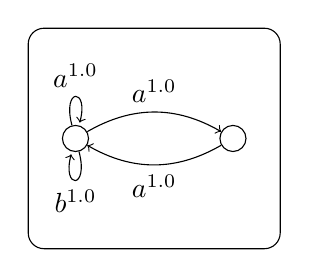
\begin{tikzpicture}
            \graphbox{}{0mm}{0mm}{32mm}{28mm}{-10mm}{-14mm}{
                \node[draw,circle] (1) at (0,0) {};
                \node[draw,circle] (2) at (2,0) {};
                \draw[->] (1) edge[loop above] node[midway, above] {$a^{1.0}$} (1) ;
                \draw[->] (1) edge[loop below] node[midway, below] {$b^{1.0}$} (1) ;
                \draw[->] (1) edge[bend left] node[midway, above] {$a^{1.0}$}  (2)  ;
                \draw[->] (2) edge[bend left] node[midway, below] {$a^{1.0}$} (1)   ;
            }
        \end{tikzpicture}
    \end{center}
\end{frame}

\begin{frame}{Weight $w_T(h)$ of Morphism $h : L \to T$}
 $w_T(h)$ : the product of the weights of the edges of $\opn{Im}(h)$
 \newline 
 \newline
 Example:
    
    \resizebox{0.6\textwidth}{!}{
        \begin{tikzpicture}
          \graphbox{\( L \)}{-50mm}{0mm}{40mm}{39mm}{2mm}{-6mm}{
            \coordinate (o) at (0mm,-10mm); 
            \node[draw,circle] (l1) at ($(o)+(-10mm,0mm)$) {1};
            \node[draw,circle] (l2) at ($(l1)+(2,0)$) {2};
            \node[draw,circle] (l3) at ($(l1) + (1,0)$) {3};
            \draw[] (l1) -- (l3) node[midway,above] {a};
            \draw[] (l3) -- (l2) node[midway,above] {a};
        } 
            \graphbox{$T$}{0mm}{0mm}{40mm}{39mm}{-10mm}{-17mm}{
                \node[draw,circle] (1) at (0,0) {$1\ 2$};
                \node[draw,circle] (2) at (2,0) {3};
                \draw[->] (1) edge[loop above] node[midway, above] {$a^{1.0}$} (1);
                \draw[->] (1) edge[loop below] node[midway, below] {$b^{1.0}$} (1);
                \draw[->,red] (1) edge[bend left] node[midway, above] {$a^{1.0}$}  (2);
                \draw[->,red] (2) edge[bend left] node[midway, below] {$a^{1.0}$} (1);
            }
            \node () at (-5mm,-15mm) {$\overset{h}{\to}$};
        \end{tikzpicture}
        }

        $ w_T(h) = 1.0 * 1.0 = 1.0$

   
\end{frame}
 

\begin{frame}{Weight $w_T$ of Graph $L$}
 $w_T(L)$: the sum of the weights $w_T(h)$ of all morphisms \( h : L \to T \)

Example : 

        \resizebox{0.3\textwidth}{!}{
              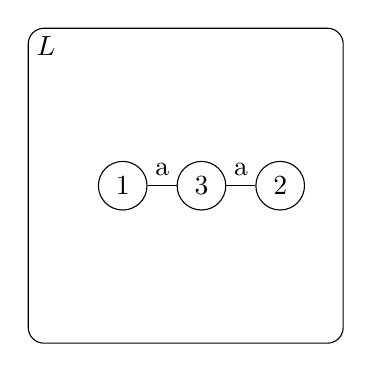
\begin{tikzpicture}
                            \graphbox{\(L\)}{-50mm}{0mm}{40mm}{40mm}{2mm}{-10mm}{
                            \coordinate (o) at (0mm,-10mm); 
                            \node[draw,circle] (l1) at ($(o)+(-10mm,0mm)$) {1};
                            \node[draw,circle] (l2) at ($(l1)+(2,0)$) {2};
                            \node[draw,circle] (l3) at ($(l1) + (1,0)$) {3};
                            \draw[] (l1) -- (l3) node[midway,above] {a};
                            \draw[] (l3) -- (l2) node[midway,above] {a};
                        } 
          \end{tikzpicture}
        }
      \resizebox{0.3\textwidth}{!}{
          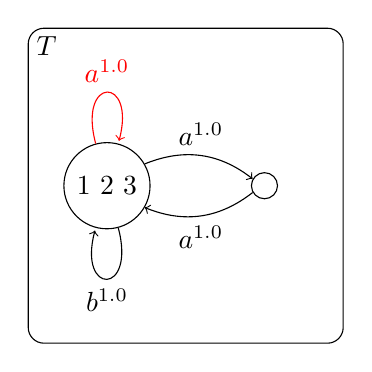
\begin{tikzpicture}
              \graphbox{$T$}{0mm}{0mm}{40mm}{40mm}{-10mm}{-20mm}{
                  \node[draw,circle] (1) at (0,0) {$1\ 2\ 3$};
                  \node[draw,circle] (2) at (2,0) {};
                  \draw[->,red] (1) edge[loop above] node[midway, above] {$a^{1.0}$} (1) ;
                  \draw[->] (1) edge[loop below] node[midway, below] {$b^{1.0}$} (1) ;
                  \draw[->] (1) edge[bend left] node[midway, above] {$a^{1.0}$}  (2)  ;
                  \draw[->] (2) edge[bend left] node[midway, below] {$a^{1.0}$} (1)   ;(1)   ;
              }
          \end{tikzpicture}
          }
        \resizebox{0.3\textwidth}{!}{
        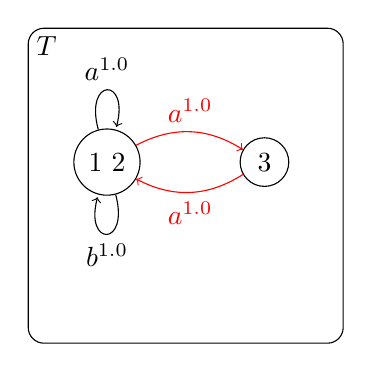
\begin{tikzpicture}
            \graphbox{$T$}{0mm}{0mm}{40mm}{40mm}{-10mm}{-17mm}{
                \node[draw,circle] (1) at (0,0) {$1\ 2$};
                \node[draw,circle] (2) at (2,0) {3};
                \draw[->] (1) edge[loop above] node[midway, above] {$a^{1.0}$} (1) ;
                \draw[->] (1) edge[loop below] node[midway, below] {$b^{1.0}$} (1) ;
                \draw[->,red] (1) edge[bend left] node[midway, above] {$a^{1.0}$}  (2)  ;
                \draw[->,red] (2) edge[bend left] node[midway, below] {$a^{1.0}$} (1)   ;
            }
        \end{tikzpicture}
        }
        \resizebox{0.3\textwidth}{!}{
        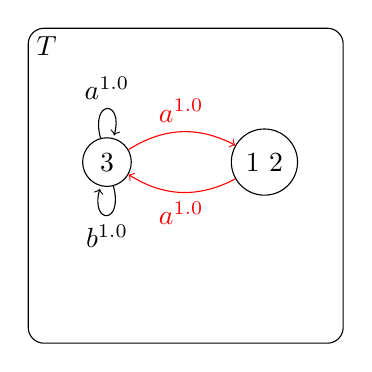
\begin{tikzpicture}
            \graphbox{$T$}{0mm}{0mm}{40mm}{40mm}{-10mm}{-17mm}{
                \node[draw,circle] (1) at (0,0) {3};
                \node[draw,circle] (2) at (2,0) {$1\ 2$};
                \draw[->] (1) edge[loop above] node[midway, above] {$a^{1.0}$} (1) ;
                \draw[->] (1) edge[loop below] node[midway, below] {$b^{1.0}$} (1) ;
                \draw[->,red] (1) edge[bend left] node[midway, above] {$a^{1.0}$}  (2)  ;
                \draw[->,red] (2) edge[bend left] node[midway, below] {$a^{1.0}$} (1);
            }
        \end{tikzpicture}
        }
        \resizebox{0.3\textwidth}{!}{
            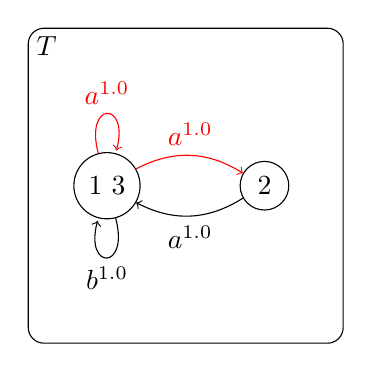
\begin{tikzpicture}
                \graphbox{$T$}{0mm}{0mm}{40mm}{40mm}{-10mm}{-20mm}{
                    \node[draw,circle] (1) at (0,0) {$1\ 3$};
                    \node[draw,circle] (2) at (2,0) {$2$};
                    \draw[->,red] (1) edge[loop above] node[midway, above] {$a^{1.0}$} (1) ;
                    \draw[->] (1) edge[loop below] node[midway, below] {$b^{1.0}$} (1);
                    \draw[->,red] (1) edge[bend left] node[midway, above] {$a^{1.0}$}  (2);
                    \draw[->] (2) edge[bend left] node[midway, below] {$a^{1.0}$} (1);
                }
            \end{tikzpicture}
            }
        \resizebox{0.3\textwidth}{!}{
        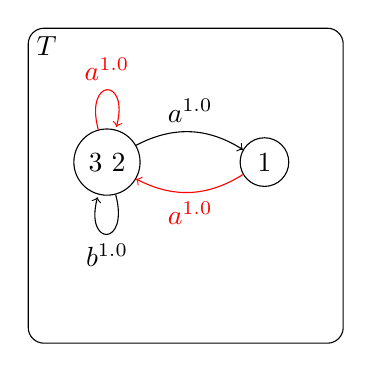
\begin{tikzpicture}
            \graphbox{$T$}{0mm}{0mm}{40mm}{40mm}{-10mm}{-17mm}{
                \node[draw,circle] (1) at (0,0) {$3\ 2$};
                \node[draw,circle] (2) at (2,0) {$1$};
                \draw[->,red] (1) edge[loop above] node[midway, above] {$a^{1.0}$} (1) ;
                \draw[->] (1) edge[loop below] node[midway, below] {$b^{1.0}$} (1) ;
                \draw[->] (1) edge[bend left] node[midway, above] {$a^{1.0}$}  (2)  ;
                \draw[->,red] (2) edge[bend left] node[midway, below] {$a^{1.0}$} (1);
            }
        \end{tikzpicture}
        }

% \begin{center}
%       \resizebox{0.49\textwidth}{!}{
%           \begin{tikzpicture}
%             \graphbox{\(L\)}{-50mm}{0mm}{40mm}{40mm}{2mm}{-10mm}{
%               \coordinate (o) at (0mm,-10mm); 
%               \node[draw,circle] (l1) at ($(o)+(-10mm,0mm)$) {1};
%               \node[draw,circle] (l2) at ($(l1)+(2,0)$) {2};
%               \node[draw,circle] (l3) at ($(l1) + (1,0)$) {3};
%               \draw[] (l1) -- (l3) node[midway,above] {a};
%               \draw[] (l3) -- (l2) node[midway,above] {a};
%           } 
%               \graphbox{$T$}{0mm}{0mm}{40mm}{40mm}{-10mm}{-20mm}{
%                   \node[draw,circle] (1) at (0,0) {$1\ 2\ 3$};
%                   \node[draw,circle] (2) at (2,0) {};
%                   \draw[->,red] (1) edge[loop above] node[midway, above] {$a^{1.0}$} (1) ;
%                   \draw[->] (1) edge[loop below] node[midway, below] {$b^{1.0}$} (1) ;
%                   \draw[->] (1) edge[bend left] node[midway, above] {$a^{1.0}$}  (2)  ;
%                   \draw[->] (2) edge[bend left] node[midway, below] {$a^{1.0}$} (1)   ;(1)   ;
%               }
%               \node () at (-5mm,-15mm) {$\overset{h_{11}^1}{\to}$};
%           \end{tikzpicture}
%           }
%         \resizebox{0.49\textwidth}{!}{
%         \begin{tikzpicture}
%           \graphbox{\( L \)}{-50mm}{0mm}{40mm}{40mm}{2mm}{-6mm}{
%             \coordinate (o) at (0mm,-10mm); 
%             \node[draw,circle] (l1) at ($(o)+(-10mm,0mm)$) {1};
%             \node[draw,circle] (l2) at ($(l1)+(2,0)$) {2};
%             \node[draw,circle] (l3) at ($(l1) + (1,0)$) {3};
%             \draw[] (l1) -- (l3) node[midway,above] {a};
%             \draw[] (l3) -- (l2) node[midway,above] {a};
%         } 
%             \graphbox{$T$}{0mm}{0mm}{40mm}{40mm}{-10mm}{-17mm}{
%                 \node[draw,circle] (1) at (0,0) {$1\ 2$};
%                 \node[draw,circle] (2) at (2,0) {3};
%                 \draw[->] (1) edge[loop above] node[midway, above] {$a^{1.0}$} (1) ;
%                 \draw[->] (1) edge[loop below] node[midway, below] {$b^{1.0}$} (1) ;
%                 \draw[->,red] (1) edge[bend left] node[midway, above] {$a^{1.0}$}  (2)  ;
%                 \draw[->,red] (2) edge[bend left] node[midway, below] {$a^{1.0}$} (1)   ;
%             }
%             \node () at (-5mm,-15mm) {$\overset{h_{11}^2}{\to}$};
%         \end{tikzpicture}
%         }
%       \end{center}
%       \begin{center}
%         \resizebox{0.49\textwidth}{!}{
%         \begin{tikzpicture}
%           \graphbox{\( L \)}{-50mm}{0mm}{40mm}{40mm}{2mm}{-6mm}{
%             \coordinate (o) at (0mm,-10mm); 
%             \node[draw,circle] (l1) at ($(o)+(-10mm,0mm)$) {1};
%             \node[draw,circle] (l2) at ($(l1)+(2,0)$) {2};
%             \node[draw,circle] (l3) at ($(l1) + (1,0)$) {3};
%             \draw[] (l1) -- (l3) node[midway,above] {a};
%             \draw[] (l3) -- (l2) node[midway,above] {a};
%         } 
%             \graphbox{$T$}{0mm}{0mm}{40mm}{40mm}{-10mm}{-17mm}{
%                 \node[draw,circle] (1) at (0,0) {3};
%                 \node[draw,circle] (2) at (2,0) {$1\ 2$};
%                 \draw[->] (1) edge[loop above] node[midway, above] {$a^{1.0}$} (1) ;
%                 \draw[->] (1) edge[loop below] node[midway, below] {$b^{1.0}$} (1) ;
%                 \draw[->,red] (1) edge[bend left] node[midway, above] {$a^{1.0}$}  (2)  ;
%                 \draw[->,red] (2) edge[bend left] node[midway, below] {$a^{1.0}$} (1);
%             }
%             \node () at (-5mm,-15mm) {$\overset{h_{22}^1}{\to}$};
%         \end{tikzpicture}
%         }
%         \resizebox{0.49\textwidth}{!}{
%             \begin{tikzpicture}
%               \graphbox{\(L\)}{-50mm}{0mm}{40mm}{40mm}{2mm}{-10mm}{
%                 \coordinate (o) at (0mm,-10mm); 
%                 \node[draw,circle] (l1) at ($(o)+(-10mm,0mm)$) {1};
%                 \node[draw,circle] (l2) at ($(l1)+(2,0)$) {2};
%                 \node[draw,circle] (l3) at ($(l1) + (1,0)$) {3};
%                 \draw[] (l1) -- (l3) node[midway,above] {a};
%                 \draw[] (l3) -- (l2) node[midway,above] {a};
%             } 
%                 \graphbox{$T$}{0mm}{0mm}{40mm}{40mm}{-10mm}{-20mm}{
%                     \node[draw,circle] (1) at (0,0) {$1\ 3$};
%                     \node[draw,circle] (2) at (2,0) {$2$};
%                     \draw[->,red] (1) edge[loop above] node[midway, above] {$a^{1.0}$} (1) ;
%                     \draw[->] (1) edge[loop below] node[midway, below] {$b^{1.0}$} (1);
%                     \draw[->,red] (1) edge[bend left] node[midway, above] {$a^{1.0}$}  (2);
%                     \draw[->] (2) edge[bend left] node[midway, below] {$a^{1.0}$} (1);
%                 }
%                 \node () at (-5mm,-15mm) {$\overset{h_{12}^1}{\to}$};
%             \end{tikzpicture}
%             }
%       \end{center}
%       \begin{center}
%         \resizebox{0.49\textwidth}{!}{
%         \begin{tikzpicture}
%           \graphbox{\( L \)}{-50mm}{0mm}{40mm}{40mm}{2mm}{-6mm}{
%             \coordinate (o) at (0mm,-10mm); 
%             \node[draw,circle] (l1) at ($(o)+(-10mm,0mm)$) {1};
%             \node[draw,circle] (l2) at ($(l1)+(2,0)$) {2};
%             \node[draw,circle] (l3) at ($(l1) + (1,0)$) {3};
%             \draw[] (l1) -- (l3) node[midway,above] {a};
%             \draw[] (l3) -- (l2) node[midway,above] {a};
%         } 
%             \graphbox{$T$}{0mm}{0mm}{40mm}{40mm}{-10mm}{-17mm}{
%                 \node[draw,circle] (1) at (0,0) {$3\ 2$};
%                 \node[draw,circle] (2) at (2,0) {$1$};
%                 \draw[->,red] (1) edge[loop above] node[midway, above] {$a^{1.0}$} (1) ;
%                 \draw[->] (1) edge[loop below] node[midway, below] {$b^{1.0}$} (1) ;
%                 \draw[->] (1) edge[bend left] node[midway, above] {$a^{1.0}$}  (2)  ;
%                 \draw[->,red] (2) edge[bend left] node[midway, below] {$a^{1.0}$} (1);
%             }
%             \node () at (-5mm,-15mm) {$\overset{h_{21}^1}{\to}$};
%         \end{tikzpicture}
%         }
%         \resizebox{0.49\textwidth}{!}{
%             \begin{tikzpicture}
%               \phantom{\graphbox{\(L\)}{-50mm}{0mm}{40mm}{40mm}{2mm}{-10mm}{
%                 \coordinate (o) at (0mm,-10mm); 
%                 \node[draw,circle] (l1) at ($(o)+(-10mm,0mm)$) {1};
%                 \node[draw,circle] (l2) at ($(l1)+(2,0)$) {2};
%                 \node[draw,circle] (l3) at ($(l1) + (1,0)$) {3};
%                 \draw[] (l1) -- (l3) node[midway,above] {a};
%                 \draw[] (l3) -- (l2) node[midway,above] {a};
%             } 
%                 \graphbox{$T$}{0mm}{0mm}{40mm}{40mm}{-10mm}{-20mm}{
%                     \node[draw,circle] (1) at (0,0) {$1\ 3$};
%                     \node[draw,circle] (2) at (2,0) {$2$};
%                     \draw[->,red] (1) edge[loop above] node[midway, above] {$a^{1.0}$} (1) ;
%                     \draw[->] (1) edge[loop below] node[midway, below] {$b^{1.0}$} (1);
%                     \draw[->,red] (1) edge[bend left] node[midway, above] {$a^{1.0}$}  (2);
%                     \draw[->] (2) edge[bend left] node[midway, below] {$a^{1.0}$} (1);
%                 }
%                 \node () at (-5mm,-15mm) {$\overset{h_{12}^1}{\to}$};
%               }
%             \end{tikzpicture}
%             }
%       \end{center}
      
      $w_T(L) = 1.0 + 1.0 + 1.0 + 1.0 + 1.0 = 5.0$
\end{frame}


\begin{frame}{Not every graph can be a weighted type graph}
  $\mathcal{R}$ : rewriting system 

  $T$ : graph  

  There must be a morphism $\alert{c} : L \to T$ such that

  For every rewriting step $G \Rightarrow_\mathcal{R} H$, defined by

      \begin{center}
        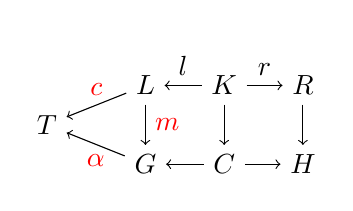
\begin{tikzpicture}[rotate=90]
          \node (I) {$K$}; 
          \node (L) [left of=I] {$L$};
          \node (R) [right of=I] {$R$};
          \node (G) [below of=L] {$G$};
          \node (C) [below of=I] {$C$};
          \node (H) [below of=R] {$H$};
          \node (T) [left=of $(L)!0.5!(G)$] {$T$};
          \draw [->] (L) to  node [label, above,red] {$c$}  (T);
          \draw [->] (G) to  node [label, below,red] {$\alpha$} (T);
          \draw [->] (I) to node [label, above] {$l$} (L);
          \draw [->] (I) to node [label,above] {$r$} (R);
          \draw [->] (L) to node [label, right,red] {$m$} (G);
          \draw [->] (I) to (C);
          \draw [->] (R) to (H);
          \draw [->] (C) to (G);
          \draw [->] (C) to (H);
        \end{tikzpicture}
      \end{center}
  there is a morphism $\alert{\alpha} : G \to T$ such that \alert{$c = \alpha \circ m$}.

  To \alert{guarantee}: $w(G)$ is defined and $w(G) \geq 0$, for all $G \Rightarrow H$
\end{frame}

\begin{frame}{Example}
  
 

  \begin{center} 
      \resizebox{0.9\textwidth}{!}{
      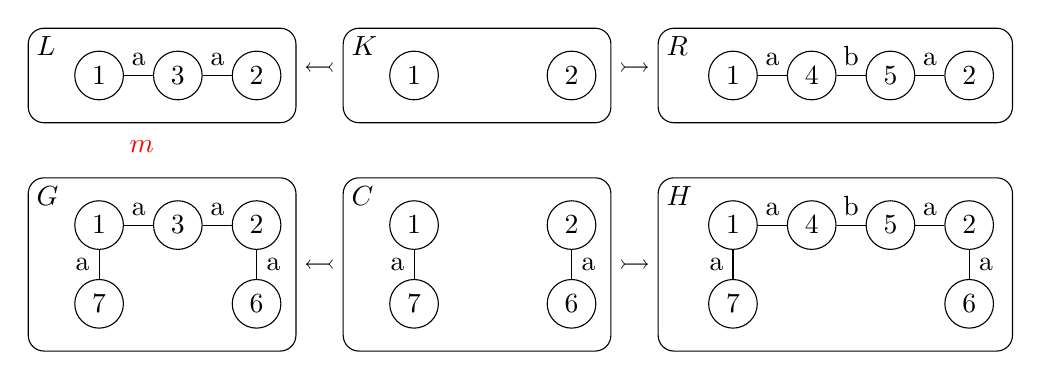
\begin{tikzpicture}
          \graphbox{\( L \)}{0mm}{-3mm}{34mm}{12mm}{2mm}{2mm}{
              \coordinate (o) at (0mm,-8mm); 
              \node[draw,circle] (l1) at ($(o)+(-10mm,0mm)$) {1};
              \node[draw,circle] (l2) at ($(l1)+(2,0)$) {2};
              \node[draw,circle] (l3) at ($(l1) + (1,0)$) {3};
              \draw[] (l1) -- (l3) node[midway,above] {a};
              \draw[] (l3) -- (l2) node[midway,above] {a};
          } 
          \graphbox{\( K \)}{40mm}{-3mm}{34mm}{12mm}{2mm}{2mm}{
              \coordinate (o) at (0mm,-8mm); 
              \node[draw,circle] (l1) at ($(o)+(-10mm,0mm)$) {1};
              \node[draw,circle] (l2) at ($(l1)+(2,0)$) {2};
          }  
          \graphbox{\( R \)}{80mm}{-3mm}{45mm}{12mm}{2mm}{2mm}{
              \coordinate (o) at (-5mm,-8mm); 
              \node[draw,circle] (l1) at ($(o)+(-10mm,0mm)$) {1};
              \node[draw,circle] (l2) at ($(l1)+(3,0)$) {2};
              \node[draw,circle] (l3) at ($(l1) + (1,0)$) {4};
              \node[draw,circle] (l4) at ($(l1) + (2,0)$) {5};
              \draw[ ] (l1) -- (l3) node[midway,above] {a};
              \draw[ ] (l3) -- (l4) node[midway,above] {b};
              \draw[ ] (l4) -- (l2) node[midway,above] {a};
          }    
          \graphbox{\( G \)}{0mm}{-22mm}{34mm}{22mm}{2mm}{-3mm}{
              \coordinate (o) at (0mm,-3mm); 
              \node[draw,circle] (l1) at ($(o)+(-10mm,0mm)$) {1};
              \node[draw,circle] (l2) at ($(l1)+(2,0)$) {2};
              \node[draw,circle] (l3) at ($(l1) + (1,0)$) {3};
              \node[draw,circle] (l4) at ($(l2) + (0,-1)$) {6};
              \draw[] (l1) -- (l3) node[midway,above] {a};
              \draw[] (l3) -- (l2) node[midway,above] {a};
              \draw[ ] (l2) -- (l4) node[midway,right] {a};
              \node[draw,circle] (l6) at ($(l1) + (0,-1)$) {7};
              \draw[] (l1) -- (l6) node[midway,left] {a};
          }    
          \graphbox{\( C  \)}{40mm}{-22mm}{34mm}{22mm}{2mm}{-3mm}{
              \coordinate (o) at (0mm,-3mm); 
              \node[draw,circle] (l1) at ($(o)+(-10mm,0mm)$) {1};
              \node[draw,circle] (l2) at ($(l1)+(2,0)$) {2};
              \node[draw,circle] (l4) at ($(l2) + (0,-1)$) {6};
              \draw[ ] (l2) -- (l4) node[midway,right] {a};
              \node[ draw,circle] (l6) at ($(l1) + (0,-1)$) {7};
              \draw[ ] (l1) -- (l6) node[midway,left] {a};
          }    
          \graphbox{\( H \)}{80mm}{-22mm}{45mm}{22mm}{2mm}{-3mm}{
              \coordinate (o) at (-5mm,-3mm); 
              \node[draw,circle] (l1) at ($(o)+(-10mm,0mm)$) {1};
              \node[draw,circle] (l2) at ($(l1)+(3,0)$) {2};
              \node[draw,circle] (l3) at ($(l1) + (1,0)$) {4};
              \node[draw,circle] (l4) at ($(l1) + (2,0)$) {5};
              \node[ draw,circle] (l5) at ($(l2) + (0,-1)$) {6};
              \node[ draw,circle] (l6) at ($(l1) + (0,-1)$) {7};
              \draw[ ] (l1) -- (l6) node[midway,left] {a};
              \draw[] (l1) -- (l3) node[midway,above] {a};
              \draw[] (l3) -- (l4) node[midway,above] {b};
              \draw[ ] (l4) -- (l2) node[midway,above] {a};
              \draw[ ] (l2) -- (l5) node[midway,right] {a};
          }    
          % \graphbox{$T$}{40mm}{-50mm}{60mm}{60mm}{-10mm}{-17mm}{
          %     % \node[draw,circle] (1) at (0,0) {$1\ 2\ 3$};
          %     % \node[draw,circle] (2) at (2,0) {};
          %     \coordinate (o) at (2mm,-12mm); 
          %     \node[draw,circle] (1) at ($(o)+(0,0mm)$) {$\substack{1\ 2\ 3\\ 6\ 7}$};
          %     \node[draw,circle] (2) at ($(o)+(2,0)$) {};
          %     \draw[->] (1) edge[loop above] node[midway, above] {$a^{1.0}$} (1) ;
          %     \draw[->] (1) edge[loop below] node[midway, below] {$b^{1.0}$} (1) ;
          %     \draw[->] (1) edge[bend left] node[midway, above] {$a^{1.0}$}  (2)  ;
          %     \draw[->] (2) edge[bend left] node[midway, below] {$a^{1.0}$} (1)   ;
          % }
          % \node () at (30mm,-55mm) {$\alpha \searrow$};
          \node () at (37mm,-8mm) {\( \leftarrowtail \)}; % K -> L
          \node () at (77mm,-8mm) {\( \rightarrowtail \)}; % K -> R
          \node () at (15mm,-18mm) {\( \textcolor{red}{m}\ \downarrowtail \)};
          \node () at (37mm,-33mm) {\( \leftarrowtail \)};
          \node () at (58mm,-18mm) {\( \downarrowtail \)};
          \node () at (102mm,-18mm) {\( \downarrowtail \)};
          \node () at (77mm,-33mm) {\( \rightarrowtail \)}; % C -> H
      \end{tikzpicture}
      }
  \end{center}

  \begin{center} 
      \resizebox{0.7\textwidth}{!}{
      \begin{tikzpicture}
          \graphbox{\( L \)}{0mm}{-3mm}{34mm}{12mm}{2mm}{2mm}{
              \coordinate (o) at (0mm,-8mm); 
              \node[draw,circle] (l1) at ($(o)+(-10mm,0mm)$) {1};
              \node[draw,circle] (l2) at ($(l1)+(2,0)$) {2};
              \node[draw,circle] (l3) at ($(l1) + (1,0)$) {3};
              \draw[] (l1) -- (l3) node[midway,above] {a};
              \draw[] (l3) -- (l2) node[midway,above] {a};
          } 
          \graphbox{\( G \)}{0mm}{-22mm}{34mm}{22mm}{2mm}{-3mm}{
              \coordinate (o) at (0mm,-3mm); 
              \node[draw,circle] (l1) at ($(o)+(-10mm,0mm)$) {1};
              \node[draw,circle] (l2) at ($(l1)+(2,0)$) {2};
              \node[draw,circle] (l3) at ($(l1) + (1,0)$) {3};
              \node[draw,circle] (l4) at ($(l2) + (0,-1)$) {6};
              \draw[] (l1) -- (l3) node[midway,above] {a};
              \draw[] (l3) -- (l2) node[midway,above] {a};
              \draw[ ] (l2) -- (l4) node[midway,right] {a};
              \node[draw,circle] (l6) at ($(l1) + (0,-1)$) {7};
              \draw[] (l1) -- (l6) node[midway,left] {a};
          }    
          \graphbox{$T$}{-60mm}{-3mm}{40mm}{40mm}{-10mm}{-17mm}{
              % \node[draw,circle] (1) at (0,0) {$1\ 2\ 3$};
              % \node[draw,circle] (2) at (2,0) {};
              \coordinate (o) at (4mm,-2mm); 
              \node[draw,circle] (1) at ($(o)+(0,0mm)$) {$\substack{1\\2\ 3\\ 6\ 7}$};
              \node[draw,circle] (2) at ($(o)+(2,0)$) {};
              \draw[->] (1) edge[loop above] node[midway, above] {$a^{1.0}$} (1) ;
              \draw[->] (1) edge[loop below] node[midway, below] {$b^{1.0}$} (1) ;
              \draw[->] (1) edge[bend left] node[midway, above] {$a^{1.0}$}  (2)  ;
              \draw[->] (2) edge[bend left] node[midway, below] {$a^{1.0}$} (1)   ;
          }
          \node () at (-10mm,-27mm) {$\textcolor{red}{\alpha} \nwarrow$};
          \node () at (15mm,-18mm) {\( \textcolor{red}{m}\ \downarrowtail \)};
          \node () at (-10mm,-10mm) {\(\textcolor{red}{c}\ \swarrow \)};
      \end{tikzpicture}
      }
  \end{center}
\end{frame}

% \begin{frame}{Condition on Weighted Type Graph: for every rewriting step $G \Rightarrow H$, there exists a morphism $h : G \to T$.}
  

%   Consequence: for all $G \Rightarrow H$, $G$ has a weight and $w(G) \geq 0$.
%   % \begin{definition}
%   %   % Let $T = (T,\mathbb{E}, S, w)$ be a type graph, \(\rho = (L \overset{l}{\leftarrow} K \overset{r}{\rightarrow} R ) \) a DPO rewriting rule and $\mathfrak{F}$ a rewriting framework. 
%   %   A \textbf{context closure} for a rule $\rho$ and a $T$ is a morphism $c:L \rightarrow T$ such that for every possible DPO diagram depicted below,
%   %   there exists $\alpha : G \rightarrow T$ such that $m \star \alpha = c$.
%   %   \begin{center}
%   %       \begin{tikzpicture}[rotate=90]
%   %         \node (I) {$K$}; 
%   %         \node (L) [left of=I] {$L$};
%   %         \node (R) [right of=I] {$R$};
%   %         \node (G) [below of=L] {$G$};
%   %         \node (C) [below of=I] {$C$};
%   %         \node (H) [below of=R] {$H$};
%   %         \node (T) [left=of $(L)!0.5!(G)$] {$T$};
%   %         \draw [->] (L) to  node [label, above] {$c$}  (T);
%   %         \draw [->] (G) to  node [label, below] {$\alpha$} (T);
%   %         \draw [->] (I) to node [label, above] {$l$} (L);
%   %         \draw [->] (I) to node [label,above] {$r$} (R);
%   %         \draw [->] (L) to node [label, right] {$m$} (G);
%   %         \draw [->] (I) to (C);
%   %         \draw [->] (R) to (H);
%   %         \draw [->] (C) to (G);
%   %         \draw [->] (C) to (H);
%   %       \end{tikzpicture}
%   %     \end{center}
%   % \end{definition}
%   % Consequence:
% \end{frame}

\begin{frame}{Sufficient Termination Condition}
  Since for all $G \Rightarrow H$, $w_T(G) \geq 0$, we have the following

  \begin{proposition}
  Rule $\varphi$ terminates, if 

   \begin{enumerate}
      \item there exists $\delta \in \mathbb{R}$, $\delta > 0$
      \item $w_T(G) - w_T(H) > \delta$ for every rewriting step $G \Rightarrow_\varphi H$
   \end{enumerate} 
  \end{proposition}


   Problem : they are infinitely many rewriting steps.

   How to show the second condition?

\end{frame}


\begin{frame}{ $w_T(G) - w_T(H) > \delta$ for every rewriting step $G \Rightarrow_\varphi H$ using rule $\varphi$ if}
  %  For $G \Rightarrow H$ defined by

  %  \begin{center}
  %     \resizebox{0.3\textwidth}{!}{
  %       \begin{tikzpicture}
  %           \node (I) at (0,0) {$K$};
  %           \node (L) at (-2,0) {$L$};
  %           \node (R) at (2,0) {$R$};
  %           \node (G) at (-2,-2) {$G$};
  %           \node (C) at (0,-2) {$C$};
  %           \node (H) at (2,-2) {$H$};
  %           \draw [->] (I) to  node [midway,below] {$l$} (L);
  %           \draw [->] (I) to  node [midway,below] {$r$} (R);
  %           \draw [->] (L) to node [midway,right] {$m$} (G);
  %           \draw [->] (I) to node [midway,right] {$u$} (C);
  %           \draw [->] (R) to node [midway,left] {$m'$} (H);
  %           \draw [->] (C) to node [midway,above] {$l'$} (G);
  %           \draw [->] (C) to node [midway,above] {$r'$} (H);
  %           \node [at=($(I)!.5!(G)$)] {\normalfont PO};
  %           \node [at=($(I)!.5!(H)$)] {\normalfont PO};
  %         \end{tikzpicture}
  %       }
  % \end{center}
% It suffices to show
% \begin{theorem}
  for every $t_K: K \rightarrow T$, 
    $$ \sum_{\substack{t_L: L \rightarrow T\\ t_K =  t_L \circ l }}
        w_T(t_L) -  \sum_{\substack{t_R: R \rightarrow T\\ t_K = t_R \circ r}}
            w_T(t_R) \geq 0 $$ 

for some $t_K: K \rightarrow T$,
$$ \sum_{\substack{t_L: L \rightarrow T\\ t_K = t_L \circ l}}
        w_T(t_L) - \sum_{\substack{t_R: R \rightarrow T\\ t_K = t_R \circ r}}
            w_T(t_R) > \delta $$ 
% \end{theorem}   
% then 
%   \begin{center}
%     $w_T(G) - w_T(H) > \delta$ for every rewriting step $G \Rightarrow_\varphi H$ using rule $\varphi$
%   \end{center}
  by [Endrullis \& Overbeek 24b, Lemma 5.13]
  % \resizebox{0.9\textwidth}{!}{
  %   \begin{flalign*}
  %     w_T(G) 
  %         & = \sum_{t_K: K \rightarrow T} 
  %         \left ( \sum_{\substack{t_C: C \rightarrow T\\ t_K = u \star t_C}}
  %           w_T(t_C - u) \right ) 
  %           \times
  %         \left (\sum_{\substack{t_L: L \rightarrow T\\ t_K = t_L \circ l}}
  %         w_T(t_L) \right )
  %         \\
  %     w_T(H) 
  %         &  \preceq \sum_{t_K: K \rightarrow T} 
  %         \left ( \sum_{\substack{t_C: C \rightarrow T\\ t_K = u \star t_C}}
  %         w_T(t_C - u) \right ) 
  %         \times 
  %         \left ( \sum_{\substack{t_R: R \rightarrow T\\ t_K = t_R \circ r}}
  %             w_T(t_R) \right ) \\
  % \end{flalign*}
  % }
\end{frame}

\begin{frame}{Example}
  There are $t_K^{11}, t_K^{12}, t_K^{21}, t_K^{22}:K \rightarrow T$ as depicted below:

    \begin{center}
        \resizebox{0.49\textwidth}{!}{
            \begin{tikzpicture}
            \graphbox{\( K \)}{-50mm}{0mm}{40mm}{30mm}{2mm}{-6mm}{
                \coordinate (o) at (0mm,-10mm); 
                \node[draw,circle] (l1) at ($(o)+(-10mm,0mm)$) {1};
                \node[draw,circle] (l2) at ($(l1)+(2,0)$) {2};
                % \node[draw,circle] (l3) at ($(l1) + (1,0)$) {3};
                % \draw[] (l1) -- (l3) node[midway,above] {a};
                % \draw[] (l3) -- (l2) node[midway,above] {a};
            } 
                \graphbox{$T$}{0mm}{0mm}{40mm}{30mm}{-10mm}{-15mm}{
                    \node[draw,circle] (1) at (0,0) {$1\ 2$};
                    \node[draw,circle] (2) at (2,0) {};
                    \draw[->] (1) edge[loop above] node[midway, above] {$a$} (1) ;
                    \draw[->] (1) edge[loop below] node[midway, below] {$b$} (1) ;
                    \draw[->] (1) edge[bend left] node[midway, above] {$a$}  (2)  ;
                    \draw[->] (2) edge[bend left] node[midway, below] {$a$} (1)   ;
                }
                \node () at (-5mm,-15mm) {$\overset{t_K^{11}}{\to}$};
            \end{tikzpicture}
            } 
            \resizebox{0.49\textwidth}{!}{
            \begin{tikzpicture}
                \graphbox{\( K \)}{-50mm}{0mm}{40mm}{30mm}{2mm}{-6mm}{
                \coordinate (o) at (0mm,-10mm); 
                \node[draw,circle] (l1) at ($(o)+(-10mm,0mm)$) {1};
                \node[draw,circle] (l2) at ($(l1)+(2,0)$) {2};
                % \node[draw,circle] (l3) at ($(l1) + (1,0)$) {3};
                % \draw[] (l1) -- (l3) node[midway,above] {a};
                % \draw[] (l3) -- (l2) node[midway,above] {a};
            } 
                \graphbox{$T$}{0mm}{0mm}{40mm}{30mm}{-10mm}{-15mm}{
                    \node[draw,circle] (1) at (0,0) {$1$};
                    \node[draw,circle] (2) at (2,0) {2};
                    \draw[->] (1) edge[loop above] node[midway, above] {$a$} (1) ;
                    \draw[->] (1) edge[loop below] node[midway, below] {$b$} (1) ;
                    \draw[->] (1) edge[bend left] node[midway, above] {$a$}  (2)  ;
                    \draw[->] (2) edge[bend left] node[midway, below] {$a$} (1)   ;
                }
                \node () at (-5mm,-15mm) {$\overset{t_K^{12}}{\to}$};
            \end{tikzpicture}
            }
            \hspace{5mm}
            
            \resizebox{0.49\textwidth}{!}{
            \begin{tikzpicture}
                \graphbox{\( K \)}{-50mm}{0mm}{40mm}{30mm}{2mm}{-6mm}{
                \coordinate (o) at (0mm,-10mm); 
                \node[draw,circle] (l1) at ($(o)+(-10mm,0mm)$) {1};
                \node[draw,circle] (l2) at ($(l1)+(2,0)$) {2};
                % \node[draw,circle] (l3) at ($(l1) + (1,0)$) {3};
                % \draw[] (l1) -- (l3) node[midway,above] {a};
                % \draw[] (l3) -- (l2) node[midway,above] {a};
            } 
                \graphbox{$T$}{0mm}{0mm}{40mm}{30mm}{-10mm}{-15mm}{
                    \node[draw,circle] (1) at (0,0) {2};
                    \node[draw,circle] (2) at (2,0) {1};
                    \draw[->] (1) edge[loop above] node[midway, above] {$a$} (1) ;
                    \draw[->] (1) edge[loop below] node[midway, below] {$b$} (1) ;
                    \draw[->] (1) edge[bend left] node[midway, above] {$a$}  (2)  ;
                    \draw[->] (2) edge[bend left] node[midway, below] {$a$} (1)   ;
                }
                \node () at (-5mm,-15mm) {$\overset{t_K^{21}}{\to}$};
            \end{tikzpicture}
            }
            \resizebox{0.49\textwidth}{!}{
            \begin{tikzpicture}
                \graphbox{\( K \)}{-50mm}{0mm}{40mm}{30mm}{2mm}{-6mm}{
                \coordinate (o) at (0mm,-10mm); 
                \node[draw,circle] (l1) at ($(o)+(-10mm,0mm)$) {1};
                \node[draw,circle] (l2) at ($(l1)+(2,0)$) {2};
                % \node[draw,circle] (l3) at ($(l1) + (1,0)$) {3};
                % \draw[] (l1) -- (l3) node[midway,above] {a};
                % \draw[] (l3) -- (l2) node[midway,above] {a};
            } 
                \graphbox{$T$}{0mm}{0mm}{40mm}{30mm}{-10mm}{-15mm}{
                    \node[draw,circle] (1) at (0,0) {};
                    \node[draw,circle] (2) at (2,0) {$1\ 2$};
                    \draw[->] (1) edge[loop above] node[midway, above] {$a$} (1) ;
                    \draw[->] (1) edge[loop below] node[midway, below] {$b$} (1) ;
                    \draw[->] (1) edge[bend left] node[midway, above] {$a$}  (2)  ;
                    \draw[->] (2) edge[bend left] node[midway, below] {$a$} (1)   ;
                }
                \node () at (-5mm,-15mm) {$\overset{t_K^{22}}{\to}$};
            \end{tikzpicture}
            }
      \end{center}

      \begin{itemize} 
        \item $t_K^{11}$ : $2 - 1 = 1 > 0$ 
        \item $t_K^{12}$ : $1 - 1 = 0 \geq 0$
        \item $t_K^{21}$ : $1 - 1 = 0 \geq 0$
        \item $t_K^{22}$ : $1 - 1 = 0 \geq 0$
      \end{itemize}

      Therefore, $w_T(G) - w_T(H) \geq 2 - 1 = 1$ for every $G \Rightarrow_\varphi H$
\end{frame}   

\begin{frame}{Example : Termination using Weighted Type Graph over Real Arithmetic Semiring}
  % DPO Rewriting Rule on Edge-labeled Directed Graphs: 
  Rule $\varphi$
    \begin{center} 
      \resizebox{0.7\textwidth}{!}{
      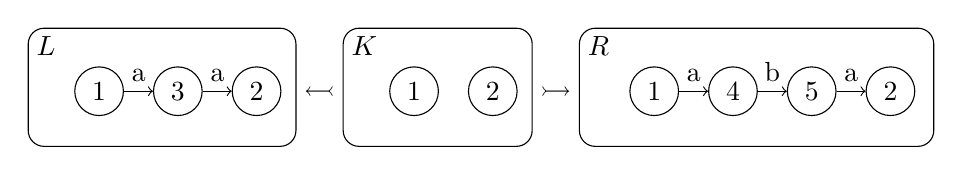
\begin{tikzpicture}
          \graphbox{$L$}{0mm}{0mm}{34mm}{15mm}{2mm}{-5mm}{
              \coordinate (o) at (0mm,-3mm); 
              \node[draw,circle] (l1) at ($(o)+(-10mm,0mm)$) {1};
              \node[draw,circle] (l2) at ($(l1)+(2,0)$) {2};
              \node[draw,circle] (l3) at ($(l1) + (1,0)$) {3};
              \draw[->] (l1) -- (l3) node[midway,above] {a};
              \draw[->] (l3) -- (l2) node[midway,above] {a};
          }     
          \graphbox{$K$}{40mm}{0mm}{24mm}{15mm}{2mm}{-5mm}{
              \coordinate (o) at (5mm,-3mm); 
              \node[draw,circle] (l1) at ($(o)+(-10mm,0mm)$) {1};
              \node[draw,circle] (l2) at ($(l1)+(1,0)$) {2};
              % \node[draw,circle] (l3) at ($(l1) + (1,0)$) {$\ $};
              % \draw[->] (l1) -- (l3) node[midway,above] {a};
              % \draw[->] (l3) -- (l2) node[midway,above] {a};
          }    
          \graphbox{$R$}{70mm}{0mm}{45mm}{15mm}{2mm}{-5mm}{
              \coordinate (o) at (-5mm,-3mm); 
              \node[draw,circle] (l1) at ($(o)+(-10mm,0mm)$) {1};
              \node[draw,circle] (l2) at ($(l1)+(3,0)$) {2};
              \node[draw,circle] (l3) at ($(l1) + (1,0)$) {4};
              \node[draw,circle] (l4) at ($(l1) + (2,0)$) {5};
              \draw[->] (l1) -- (l3) node[midway,above] {a};
              \draw[->] (l3) -- (l4) node[midway,above] {b};
              \draw[->] (l4) -- (l2) node[midway,above] {a};
          }    
          \node () at (37mm,-8mm) {$\leftarrowtail$};
          \node () at (67mm,-8mm) {$\rightarrowtail$};
          % \draw[>->] (51mm,2mm) -- (52mm,3mm);
      \end{tikzpicture}
      }
  \end{center}

  Termination proved by:
    \begin{center}
        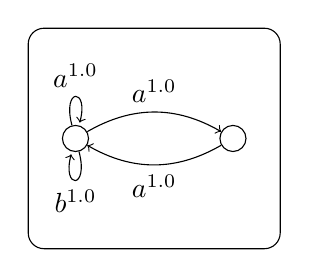
\begin{tikzpicture}
            \graphbox{}{0mm}{0mm}{32mm}{28mm}{-10mm}{-14mm}{
                \node[draw,circle] (1) at (0,0) {};
                \node[draw,circle] (2) at (2,0) {};
                \draw[->] (1) edge[loop above] node[midway, above] {$a^{1.0}$} (1) ;
                \draw[->] (1) edge[loop below] node[midway, below] {$b^{1.0}$} (1) ;
                \draw[->] (1) edge[bend left] node[midway, above] {$a^{1.0}$}  (2)  ;
                \draw[->] (2) edge[bend left] node[midway, below] {$a^{1.0}$} (1)   ;
            }
        \end{tikzpicture}
    \end{center}
    \begin{itemize}
      \item edge labels : a, b
      \item edge weights : superscripts of edge labels
      % \item weights satisfy conditions expressed as first-order formulas
    \end{itemize}
  % Existence of suitable weighted type graphs: \textcolor{red}{undecidable}
  
  % How to find a suitable weighted type graph in practice ?

\end{frame}

\begin{frame}{Concrete Semirings}
  For each existing well-founded semiring (on the left), we propose a corresponding non-well-founded semiring (on the right):

  \begin{center}
     Natural Tropical Semiring $\Leftrightarrow$ Real Tropical Semiring
  \end{center}
  \begin{center}
     Natural Arctic Semiring $\Leftrightarrow$ Real Arctic Semiring
  \end{center}
  \begin{center}
    Natural Arithmetic Semiring $\Leftrightarrow$ Real Arithmetic Semiring
  \end{center}

  natural semirings: semirings on the left,
  real semirings: semirings on the right.
\end{frame}

\begin{frame}{Searching Weighted Type Graphs over the natural vs. real semirings}
    % Searching a weighted finite graph  with 
    \begin{itemize}
      \item $k$ nodes
      \item no parallel edges of the same label from $\Sigma$
      \item weighted edges
    \end{itemize} 
  In available tools

  \begin{enumerate}
    \item Decide if $s \overset{l}{\to} t$ exists for each pair of nodes \( s, t\) and label \( l\)
    \item Assign a \crossout[red]{natural} real number as weight for each existing edge
    \item Check if the sufficient condition is satisfied
    % the weighted type graph satisfies the conditions 
    % expressed as first-order formulas in Peano arithmetic
  \end{enumerate}

  % Analyse: 
  %     \begin{itemize}
  %         % \item weights in $\mathbb{R}^+$
  %         % \item a graph $G$ is interpreted as $w_T(G) \in \mathbb{R}^+ \cup \{\infty\}$
  %         % \item $w_T(G) \in \mathbb{R}^+$ for all $G \Rightarrow H$
  %         \item terminating if there is $\delta > 0$ and 
  %             \\ \hspace{2.3cm}$w_T(G) - w_T(H) > \delta$ for all $G \Rightarrow H$
  %         \item 
    Analyse : 
      \begin{itemize}
        \item $k^2|\Sigma|$ binary variables
        \item $k^2|\Sigma|$ \crossout[red]{integer} real variables
      \end{itemize}
    
    Complexity:
      \begin{itemize}
        \item \crossout[red]{$O(2^{2k^2|\Sigma|})$} $O(2^{k^2|\Sigma|})$, or 
        \item \crossout[red]{undecidable} decidable (but double exponential)
      \end{itemize}
      % \end{itemize}
\end{frame}

\begin{frame}{Implementation, Experimental Results and Analysis}
  \alert{Implemented} in the tool LyonParallel
        \begin{itemize}
          \item supports natural and real semirings
          \item searches with different semirings in parallel and cooperates between them
          \item for edge-labeled directed graph rewriting
        \end{itemize}

  \alert{Tested} on examples from previous work:
  \begin{itemize}
    \item \alert{Acceleration} with \alert{Real Tropical} or \alert{Arctic Semiring} for most cases
    \item Many \alert{timeouts} (200 seconds) with \alert{Real Arithmetic Semiring} (double exponential complexity)
  \end{itemize}
\end{frame}

\begin{frame}{Conclusion}
  \begin{itemize}
    \item Type Graph Method 
         \begin{itemize}
          \item termination technique
          \item for DPO rewriting systems
          \item using weighted type graphs over semirings
         \end{itemize}
    \item It works with \textcolor{red}{non-well-founded} semirings
    \item \textcolor{red}{Complexity reduced}
    \item In practice: \textcolor{red}{acceleration} only with Real Tropical or Arctic Semiring
    % \item Tool: \textcolor{red}{LyonParallel} 
    %     \begin{itemize}
    %       \item supports well-founded and non-well-founded approaches
    %       \item searches with different approaches in parallel and cooperates between them
    %       \item for edge-labeled directed graph rewriting
    %     \end{itemize}
  \end{itemize}
\end{frame} 

\begin{frame}{Acknowledgements}
  \begin{itemize}
    \item Thanks to the anonymous reviewers.
    \item The termination section was inspired by a presentation by Plump (2018).
    \item Graph visualization from Endrullis \& Overbeek (2024).
    \item All concepts are from or adapted from Endrullis \& Overbeek (2024).
  \end{itemize}
\end{frame}

\end{document} 